\section{The corner bound and unrestricted intersection cuts}
\label{fd:section}

Fix a closed set $S\subseteq\R^k$, a point $\sbar\notin S$, and a matrix
$P=[p_1,\ldots,p_N]\in\R^{k\times N}$. The nonnegative coordinates
$\lambda$ describe a corner $\sbar+P\R_+^N$. They may be the coordinates of
a simplicial LP basis before projection onto the constraint variables;
the projected columns of $P$ need not be independent. For reduced costs
$\rc\ge0$, define
\begin{equation}\label{fd:corner-def}
 X=\{\lambda\ge0:\sbar+P\lambda\in S\},\qquad
 \zK(\rc)=\inf_{\lambda\in X}\rc^T\lambda,
\end{equation}
with the infimum of the empty set equal to $+\infty$.

A closed convex set $C$ is \emph{$S$-free} if
$\intt C\cap S=\varnothing$. We use sets with $\sbar\in\intt C$. Their
ray steps and cut coefficients are
\[
 \alpha_j(C)=\sup\{t\ge0:\sbar+tp_j\in C\},\qquad
 a_j(C)=1/\alpha_j(C),\qquad 1/(+\infty)=0.
\]
The intersection cut and its corner value are
\begin{equation}\label{fd:cut-value}
 a(C)^T\lambda\ge1,\qquad
 z_C(\rc)=\min_{j:a_j(C)>0}\frac{\omega_j}{a_j(C)}.
\end{equation}
If all coefficients vanish, the cut is infeasible and its value is
$+\infty$. The restriction $a_j>0$ avoids an ambiguous product
$0\cdot\infty$ when a zero-cost ray has infinite step.

To see validity, a point with $a(C)^T\lambda<1$ is a convex combination
of finite ray exits and the apex, with positive weight on the apex,
plus recession directions corresponding to infinite steps. It therefore
lies in $\intt C$. In particular, $z_C(\rc)\le\zK(\rc)$.
For positive costs and $t>0$, introduce the objective simplex
\begin{equation}\label{fd:simplex-def}
 T_t=\sbar+P\{\lambda\ge0:\rc^T\lambda\le t\}
 =\conv\left\{\sbar,\sbar+\frac{t}{\omega_j}p_j:1\le j\le N\right\}.
\end{equation}
Then $z_C(\rc)\ge t$ exactly when $T_t\subseteq C$. Equivalently,
$a_j(C)\le\omega_j/t$ for every $j$; the resulting cut dominates the
objective-parallel inequality $\rc^T\lambda\ge t$ on the orthant.

\begin{theorem}[Unrestricted single-cut value]\label{fd:single-cut}
If $\rc>0$, every nonempty $X$ has an attained, finite, positive corner
value, and
\[
 \sup_{C:\sbar\in\intt C, C\ S\text{-free}}z_C(\rc)=\zK(\rc).
\]
This equality includes the value $+\infty$. The supremum is unchanged
if only maximal $S$-free sets are used.
\end{theorem}
\begin{proof}
The closed set $X$ avoids zero, and positive-cost sublevel sets in the
orthant are compact. This proves attainment and positivity when $X$ is
nonempty. For any finite $0<t<\zK(\rc)$, the compact set $T_t$ misses
$S$, so $T_t+\delta B$ also misses $S$ for a sufficiently small
$\delta>0$, where $B$ is the closed unit ball. It is a free neighbourhood
of the apex and contains $T_t$, proving a cut value at least $t$.
Let $t$ increase to the corner value, or increase without bound when
$X$ is empty. Every full-dimensional free set extends to a maximal one:
for a nested chain, the interior of the closed union is the union of
the interiors, as a finite simplex around an interior point can be
placed in a single chain member. Zorn's lemma applies. Enlargement
increases all ray steps.
\end{proof}

The direct proof uses genuine neighbourhoods of the apex. It also explains
why equality need only be a supremum. The sufficiency of cut-generating
functions under cone hypotheses is established by
\citet{CWY2015}, \citet{CCDLM2015}, and \citet{KKSteffy2016}; relaxed
cut-generating functions and their sufficiency are treated by
\citet{KKSteffy2016}. The following precise cone case has a short
polyhedral proof, given in \cref{fd:cone-proof}.

\begin{proposition}[The cone containment case]\label{fd:cone-attainment}
Suppose $S-\sbar\subseteq\cone(P)$. Every valid inequality
$c^T\lambda\ge1$ for $X$, with $c\ge0$, is dominated on $\R_+^N$ by
one intersection cut from a free neighbourhood of $\sbar$.
Consequently the best single-cut value is attained for every
$\rc\ge0$. The hypothesis holds in particular when $\cone(P)=\R^k$.
\end{proposition}

Without cone containment, a sufficient condition concerns the direction
in which the optimum simplex meets the boundary.
\begin{theorem}[Attainment under transversality]\label{fd:attainment}
Let $S=\{s:q(s)\le0\}$ with $q\in C^1$, $q(\sbar)>0$, and $\rc>0$.
Suppose $z=\zK(\rc)<\infty$ and every minimizing contact
$t=\sbar+P\lambda$ satisfies
\begin{equation}\label{fd:transverse-condition}
 \nabla q(t)^T(\sbar-t)>0.
\end{equation}
For sufficiently small $\delta>0$,
$C_\delta=\conv(T_z\cup B(\sbar,\delta))$ is $S$-free and has
$z_{C_\delta}(\rc)=z$. Every maximal free extension also attains $z$.
\end{theorem}
The condition says that movement from a contact toward the apex enters
the forbidden side at a positive first-order rate. Uniformity over the
compact contact set allows the apex to be thickened. A full proof,
including noninjective $P$, is in \cref{fd:attainment-proof}.
Multiplying a Fritz John system
$\sigma_0\rc+\sigma P^T\nabla q(t)-\nu=0$ by a minimizing $\lambda$
gives
$\sigma\nabla q(t)^T(\sbar-t)=\sigma_0z$.
Thus a positive objective multiplier implies \cref{fd:transverse-condition}.
The examples of \citet{KKYang2017} already show the distinction between
transverse and tangential approach; \cref{fd:attainment} states a
sufficient smooth condition for the equality case.

\begin{example}[Zero costs and non-attainment]\label{fd:boundary-examples}
For $S=\{(x,y):(x+1)y+1\le0\}$, apex zero, rays $e_1,e_2$, and
$\rc=(0,1)$, the corner is infeasible and $\zK=+\infty$, but every
intersection cut has value zero. Replacing the quadratic by
$(x+1)y+1-y^2$ gives the same single-cut value zero and the finite attained
corner value $(1+\sqrt5)/2$.

With positive costs, take
$q(x,y)=x-x^2+(1-y)^2$, the same apex and rays, and $\rc=(1,1)$.
The corner value is one, attained only at $(0,1)$, but no free
neighbourhood attains this single-cut value.
\end{example}
These quadratic examples illustrate known sufficiency failures
\citep{CCDLM2015,KKYang2017}. Exact proofs are in
\cref{fd:boundary-proof}.

\begin{theorem}[The unrestricted corner closure]\label{fd:dominant}
For every closed $S$ and every $P$,
\[
 \bigcap_C\{\lambda\ge0:a(C)^T\lambda\ge1\}
 =\mathcal D:=\cl(\conv X+\R_+^N),
\]
where $C$ ranges over all free neighbourhoods of $\sbar$.
\end{theorem}
\begin{proof}
Every cut halfspace is closed, convex, and upward closed, and contains
$X$, so it contains $\mathcal D$. If a nonnegative $\widehat\lambda$
lies outside a nonempty $\mathcal D$, strong separation and its
recession directions give $u\ge0$ with
$u^T\widehat\lambda<\inf_Xu^T\lambda$.
For sufficiently small $\epsilon>0$, the strict inequality persists
with $u+\epsilon\mathbf1$, since its infimum over $X$ cannot decrease.
\Cref{fd:single-cut} supplies a cut whose value exceeds
$(u+\epsilon\mathbf1)^T\widehat\lambda$, so this point violates that cut.
If $X$ is empty, use a positive normal and a target larger than its value
at $\widehat\lambda$. Points outside the orthant are already excluded.
\end{proof}

\subsection{How many rays must be considered?}

\begin{lemma}[Independent ray representations]\label{fd:rank-support}
Let $T\subseteq\R^k$ be closed and
$X=\{\lambda\ge0:\sbar+P\lambda\in T\}$, with $r_0=\rank P$.
Writing $X_J=X\cap\{\lambda_{J^c}=0\}$,
\[
 \conv X=\conv\!\left(\bigcup_{\substack{|J|\le r_0\\P_J\text{ injective}}}
 X_J\right)+\{\delta\ge0:P\delta=0\}.
\]
For every $\rc\ge0$, the infimum is the minimum of the support-restricted
infima over these $J$. If attained, it is attained on one such support.
\end{lemma}
\begin{proof}
For any $\lambda\in X$, the pointed fibre polyhedron
$\{\mu\ge0:P\mu=P\lambda\}$ consists of convex combinations of its
vertices plus its recession cone $\{\delta\ge0:P\delta=0\}$.
A vertex has independent supported columns, and all fibre points belong
to $X$. This proves the identity. Minimizing a nonnegative cost on a
fibre gives a vertex optimum, which proves the value and attainment claims.
\end{proof}

For $q(s)=s^TQs+b^Ts+c$, let $n_+(Q),n_-(Q),n_0(Q)$ denote its inertia.
The nonnegative part of the form yields a sharper bound.
\begin{theorem}[The inertia support bound]\label{fd:inertia}
Assume $q(\sbar)>0$, $\rc>0$, and a feasible corner. Define
\[
 \rho(q)=n_+(Q)+n_0(Q)+1-\mathbf1_{\{b\notin\operatorname{range}Q\}}.
\]
Every minimizing ray vector with independent supported columns has
at most $\rho(q)$ positive coordinates. Some minimizer therefore uses
at most $\min(\rank P,\rho(q))$ rays.
\end{theorem}
\begin{proof}
On an independent support $J$ the positive coordinates $\mu$ minimize
$\rc_J^T\mu$ subject to
$g(\mu)=\mu^TG\mu+2m^T\mu+g_0\le0$, where $G=P_J^TQP_J$.
The constraint is active. If $\nabla g\ne0$, KKT gives
$\rc_J=-\sigma\nabla g$ with $\sigma>0$, and second-order necessity
makes $Q$ nonnegative on
$V=P_J\{d:\rc_J^Td=0\}$, of dimension $|J|-1$.
This subspace lies in $\nabla q(t)^\perp$.
Its intersection with $\ker Q$ is contained in $\ker Q\cap b^\perp$,
of dimension $n_0-\mathbf1_{\{b\notin\operatorname{range}Q\}}$.
Modulo $\ker Q$, a nonnegative subspace has dimension at most $n_+$.
These dimensions give the stated bound.

If $\nabla g=0$, then $g(\mu+d)=d^TGd$. A negative direction belongs
to an open symmetric cone, which contains a direction with nonzero
cost derivative; one of its signs decreases the objective while staying
feasible. Hence $G\succeq0$. The same dimension argument now applies to
the whole $|J|$-dimensional supported subspace and gives the stronger
bound $|J|\le\rho(q)-1$.
\end{proof}

For $q=w-xy$, $n_+=n_0=1$ and $b\notin\operatorname{range}Q$, so
$\rho=2$. For strictly concave $q$ in a feasible corner, $\rho=1$, so
a first ray contact attains the corner bound. More generally, if the open complement of a
closed $S$ is convex, its closure is the unique maximal full-dimensional
free set, and its cut attains the corner value by \cref{fd:single-cut}.
This generic reverse-convex observation does not require the inertia
bound. In two variables, $\min(k,\rho)\le2$, although $\rho$ itself
can equal three.

\subsection{Algorithms and complexity}

\begin{theorem}[Fixed-parameter computation]\label{fd:algorithms}
For rational quadratic data with $q(\sbar)>0$, rational positive costs, and
$r=\min(\rank P,\rho(q))$, deciding $\zK(\rc)\le t$ for rational $t$ takes
polynomial time in the input size when $r$ is fixed. A finite positive
value can be approximated to relative accuracy $\epsilon$ in time
polynomial in the input size and $\log(1/\epsilon)$.

If $\rank P=k$, the search can instead use at most
$O(N^{\lfloor k/2\rfloor})$ independent $k$-ray cells of a refinement
of the fibre-cost normal fan, together with their supports of size at
most $r$. For $k=3$, at most $2N-4$ cells and $3N-6$ two-ray edges suffice.
\end{theorem}
\Cref{fd:algorithm-proof} gives the fixed-variable algebraic decision
argument, the initial approximation bracket, and the degeneracy-safe
normal-fan construction. Generic stationary-point formulas apply on
nonsingular faces. At most two rays admit a formula covering all singular
and tangential cases.

\begin{proposition}[An exact two-ray formula]\label{fd:two-ray}
Fix rays $i,j$ and put
$\nu(\theta)=(\theta/\omega_i,(1-\theta)/\omega_j)$ for
$0\le\theta\le1$. Write
\[
 q(\sbar+\tau P_{ij}\nu(\theta))
 =a(\theta)\tau^2+b(\theta)\tau+g_0,
 \qquad \Delta(\theta)=b(\theta)^2-4g_0a(\theta),
\]
where $g_0=q(\sbar)>0$. The two-ray value is
\[
 z_{ij}=\frac{1}{\displaystyle\max_{\substack{0\le\theta\le1\\\Delta(\theta)\ge0}}
 u_+(\theta)},\qquad
 u_+(\theta)=\frac{-b(\theta)+\sqrt{\Delta(\theta)}}{2g_0},
\]
provided the maximum is positive; otherwise $z_{ij}=+\infty$.
The maximum is obtained among the interval endpoints, real roots of $\Delta$,
and roots of $\Delta'^2-4b'^2\Delta$ and $\Delta'$, with identically vanishing
polynomials treated as in \cref{fd:two-ray-proof}.
\end{proposition}
Consequently a bilinear corner requires $O(N^2)$ such one- and two-ray
formulas. When $\rank P=3$, a three-dimensional convex-hull computation
followed by at most $4N-6$ formulas suffices. The unrestricted supremum
is attained unless some minimizing contact is the tangent first contact
of a single ray; the independent-representation argument proving this
qualification is in \cref{fd:bilinear-attainment-proof}.

\begin{theorem}[Variable-dimension hardness]\label{fd:hardness}
Computing the corner value is NP-hard when the constraint dimension is
part of the input, even with $P=I$, $\sbar=0$, and $\rc=\mathbf1$.
Rational-threshold decision is NP-hard, as is approximation within
relative error $1/(5k^2)$ in dimension $k$. By \cref{fd:single-cut}, the
same statements hold for the unrestricted best single-cut value.
\end{theorem}
The proof in \cref{fd:hardness-proof} is a Motzkin--Straus reduction.
The reduction has unbounded $\rho$ as well as unbounded dimension.
A carefully normalized efficacy optimization is also possible with the
fixed-parameter oracle; \cref{fd:efficacy} specifies the separation oracle
and metric needed for that assertion.

\subsection{A fixed-corner closure and a first-round polytope closure differ}

\begin{proposition}\label{fd:nonlocal-hull}
For a polytope $\mathcal P$ and closed $S$,
\[
 \bigcap_{C\ S\text{-free}}\conv(\mathcal P\setminus\intt C)
 =\conv(\mathcal P\cap S).
\]
\end{proposition}
This operation permits free sets unrelated to an LP basis. In contrast,
the rank-one basis intersection-cut closure intersects $\mathcal P$ with
all intersection cuts from its original feasible bases.

\begin{proposition}[A rank-one closure gap]
\label{fd:rank-one-example}
Let $\mathcal P=\conv\{(0,2),(-1/2,0),(1/2,0)\}$ and
$S=\{s:\norm{s}\ge1\}$. Put
\[
 t=\frac{1+2\sqrt{13}}{17},\qquad
 p_{1,2}=\left(\mp\frac{1-t}{2},2t\right),\qquad
 v=\left(0,\frac{1+\sqrt{13}}6\right).
\]
The rank-one basis intersection-cut closure is
$\conv\{(0,2),p_1,v,p_2\}$, strictly larger than
$\conv(\mathcal P\cap S)=\conv\{(0,2),p_1,p_2\}$.
A second round at $v$ gives the chord $p_1p_2$ and the hull.
\end{proposition}
\Cref{fd:polytope-proof} proves both propositions. The example uses
all free sets, not a restricted quadratic family. It therefore also
shows why the fixed-corner equality in \cref{fd:dominant} cannot imply
one-round convergence for a polytope.

\begin{figure}[htbp]
 \centering
 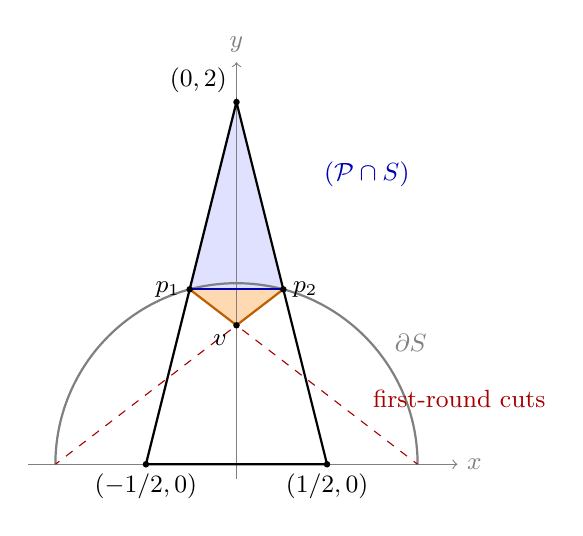
\begin{tikzpicture}[scale=2.3, every node/.style={font=\small}]
 \pgfmathsetmacro{\contactt}{(1+2*sqrt(13))/17}
 \pgfmathsetmacro{\contactx}{(1-\contactt)/2}
 \pgfmathsetmacro{\contacty}{2*\contactt}
 \pgfmathsetmacro{\closurey}{(1+sqrt(13))/6}
 \coordinate (top) at (0,2);
 \coordinate (left) at (-.5,0);
 \coordinate (right) at (.5,0);
 \coordinate (p1) at (-\contactx,\contacty);
 \coordinate (p2) at (\contactx,\contacty);
 \coordinate (v) at (0,\closurey);
 \fill[blue!12] (top)--(p1)--(p2)--cycle;
 \fill[orange!30] (p1)--(v)--(p2)--cycle;
 \draw[gray,thin,->] (-1.15,0)--(1.22,0) node[right] {$x$};
 \draw[gray,thin,->] (0,-.08)--(0,2.22) node[above] {$y$};
 \draw[gray,thick] (1,0) arc[start angle=0,end angle=180,radius=1];
 \draw[black,thick] (top)--(left)--(right)--cycle;
 \draw[red!65!black,dashed] (p1)--(1,0);
 \draw[red!65!black,dashed] (p2)--(-1,0);
 \draw[blue!70!black,thick] (p1)--(p2);
 \draw[orange!75!black,thick] (p1)--(v)--(p2);
 \foreach \point in {top,left,right,p1,p2,v}
   \fill (\point) circle[radius=.018];
 \node[above left] at (top) {$(0,2)$};
 \node[below] at (left) {$(-1/2,0)$};
 \node[below] at (right) {$(1/2,0)$};
 \node[left] at (p1) {$p_1$};
 \node[right] at (p2) {$p_2$};
 \node[below left] at (v) {$v$};
 \node[gray,above right] at (.82,.57) {$\partial S$};
 \node[blue!70!black,align=left,right] at (.43,1.6)
   {$\conv(\mathcal P\cap S)$};
 \node[red!65!black,align=left,right] at (.7,.36)
   {first-round cuts};
\end{tikzpicture}

 \caption{The unrestricted rank-one closure in
 \cref{fd:rank-one-example}. The feasible hull is blue. The first-round
 cuts also retain the orange triangle below its chord. A cut at the new
 vertex $v$ removes that triangle.}
 \label{fd:rank-one-figure}
\end{figure}
